Il seguente codice MatLab contiene la soluzione dell'$Es 4$:\\\
	\lstinputlisting[language=Matlab]{Cap_6/Es_4/Es_4.m}
nel qualche viene richiamato:\\\
	\begin{enumerate}
		\item \textbf{A = sparceMatrix(n)}\\\
			Effettua la creazione di \textit{matrici sparse} della dimensione $nXn$;\\\
		\item \textbf{x,i,B = gaussSeidel(A,b,tol,x0)}\\\
			Effettua sia il calcolo del \textit{vettore incognite} della matrice $A$, sia il numero di iterazioni impiegate, sia il calcolo di una matrice $B$ contenente il \textit{passo di ogni iterazione} con il corrispettivo \textit{valore della norma}, avendo come \textit{Input}, oltre la 	\textit{matrice}, il \textit{vettore termini noti}, e la \textit{tolleranza}, anche un \textit{vettore iniziale, in questo caso nullo}.\\\
			\lstinputlisting[language=Matlab]{Cap_6/Es_4/gaussSeidel.m}
			\begin{itemize}
				\item \textbf{u = mSolve(M,r)}\\\
					Effettua il calcolo di una matrice \textit{triangolare inferiore}.\\\
					\lstinputlisting[language=Matlab]{Cap_6/Es_4/mSolve.m}
			\end{itemize}
	\end{enumerate}
e restituisce graficamente i seguenti risultati:\\\
	\begin{figure}[H]
		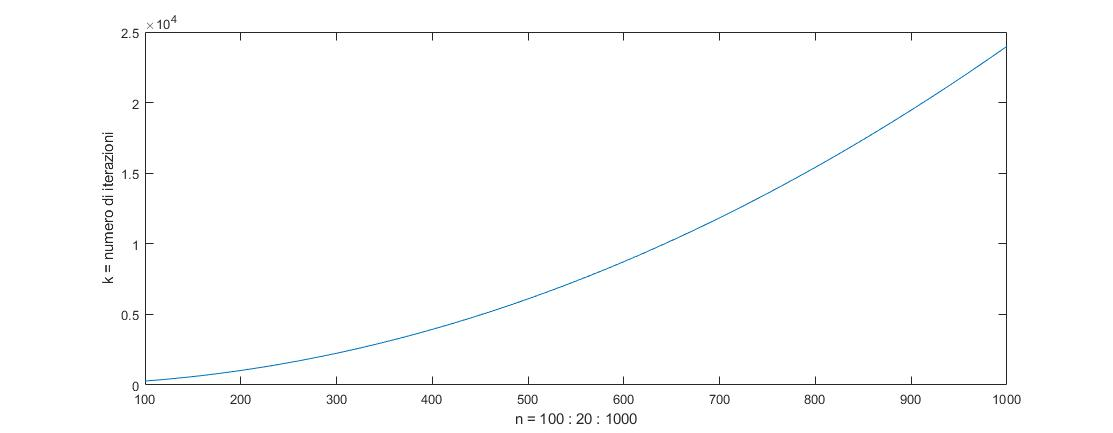
\includegraphics[width=\textwidth]{Plot/Cap_6_Es_4}
	\end{figure}
Possiamo notare come rispetto al metodo di \textit{Jacobi}, rappresentato nel grafico del precedente esercizio, in questo caso con l'utilizzo del metodo di \textit{Gauss-Seidel}, il \textit{numero di iterazione}, è circa la metà. Infatti, anche se entrambi i metodi sono convergenti, per effetto dei loro \textit{raggi spettrali} che sono $<1$ :
	\[
		\rho(M^{-1}_{GS}*N_{GS})<1 \quad \rho(M^{-1}_{J}*N_{J})<1
	\]
il metodo di \textit{Gauss-Seidel} converge prima, proprio perchè il suo \textit{raggio spettrale} è inferiore di quello del metodo di \textit{Jacobi} :
	\[
		\rho(M^{-1}_{GS}*N_{GS})<\rho(M^{-1}_{J}*N_{J})
	\]
Ciò è dovuto dal fatto, che essendo entrami i metodi basati su \textit{splitting regolari}, uno è piu efficiente dell'altro in quanto :
	\[
		0<U_{GS}=N_{GS}<N_{J}=(L+U)_{J}
	\]
